% Template for seminar reports
% Computer Vision Group, Visual Computing Institute, RWTH Aachen University
\documentclass[twoside,a4paper,10pt,DIV=12,BCOR=12mm]{scrartcl}
\usepackage[utf8]{inputenc}    % allows special symbols in LaTeX source code
\usepackage[english]{babel}    % select language of your report (use "ngerman" for German)
\usepackage[T1]{fontenc}       % font encoding, important for umlauts
\usepackage{lmodern}           % lmodern font
\usepackage{xcolor}            % use and define colors for text and images
\usepackage{graphicx}          % include images
\usepackage{booktabs}          % pretty tables
\usepackage{caption}           % captions for figures
\usepackage{subcaption}        % captions for subfigures
\usepackage{url}               % for website links
\usepackage{datetime}          % month on title page
\usepackage{hyperref}          % make references clickable
\usepackage{xspace}            % correct spaces after e.g. "e.g."
\usepackage{tikz}              % custom plots in LaTeX
\usepackage{pgfplots}          % custom function graphs in LaTeX
\usepackage{bm}                % bold math symbols
\usepackage{amsmath}           % additional math environments
\usepackage{amssymb}           % additional math symbols (includes amsfonts)
\usepackage{enumitem}          % change distances for enumerations
\usepackage{listings}          % code
\usepackage{lipsum}            % placeholder text
\usepackage{listings}
\usepackage{color}

\definecolor{dkgreen}{rgb}{0,0.6,0}
\definecolor{gray}{rgb}{0.5,0.5,0.5}
\definecolor{mauve}{rgb}{0.58,0,0.82}

\lstset{frame=tb,
  language=python,
  aboveskip=3mm,
  belowskip=3mm,
  showstringspaces=false,
  columns=flexible,
  basicstyle={\small\ttfamily},
  numbers=none,
  numberstyle=\tiny\color{gray},
  keywordstyle=\color{blue},
  commentstyle=\color{dkgreen},
  stringstyle=\color{mauve},
  breaklines=true,
  breakatwhitespace=true,
  tabsize=3
}

\newdateformat{monthyeardate}{\monthname[\THEMONTH] \THEYEAR}

\setlength{\parindent}{0pt}
\setlength{\parskip}{0pt}
\setlist{nosep}

\makeatletter
\DeclareRobustCommand\onedot{\futurelet\@let@token\@onedot}
\def\@onedot{\ifx\@let@token.\else.\null\fi\xspace}
\def\eg{{e.g}\onedot} \def\Eg{\emph{E.g}\onedot}
\def\ie{{i.e}\onedot} \def\Ie{\emph{I.e}\onedot}
\def\cf{{c.f}\onedot} \def\Cf{\emph{C.f}\onedot}
\def\etc{{etc}\onedot} \def\vs{\emph{vs}\onedot}
\def\wrt{w.r.t\onedot} \def\dof{d.o.f\onedot}
\def\etal{\emph{et al}\onedot}
\makeatother

\overfullrule=1ex

\pgfplotsset{compat=newest}


\tikzset{basic/.style={draw,fill=none,
                       text badly centered,minimum width=3em}}
\tikzset{input/.style={basic,circle,minimum width=3.5em}}
\tikzset{weights/.style={basic,rectangle,minimum width=2em}}
\tikzset{functions/.style={basic,circle, minimum width=3em}}
\newcommand{\addaxes}{\draw (0em,1em) -- (0em,-1em)
                            (-1em,0em) -- (1em,0em);}
\newcommand{\relu}{\draw[line width=1.5pt] (-1em,0) -- (0,0)
                                (0,0) -- (0.75em,0.75em);}
\newcommand{\stepfunc}{\draw[line width=1.5pt] (0.65em,0.65em) -- (0,0.65em) 
                                    -- (0,-0.65em) -- (-0.65em,-0.65em);}


% =========================================================================

\graphicspath{{pictures/}}
\setcounter{secnumdepth}{3}
\setcounter{tocdepth}{3}

% =========================================================================
\begin{document}

% Template for seminar reports
% Seminar Current Topics in Computer Vision and Machine Learning

\begin{titlepage}
\begin{center}
\ 
\vspace{3.5cm}

\textsf{
RWTH Aachen University \\
Faculty of Mathematics, Computer Science and Natural Sciences\\
Chair of Computer Science 13 (Computer Vision) \\
Prof. Dr. Bastian Leibe
}

\rule{\linewidth}{1pt}

\vspace{1.75cm}
\LARGE
\textbf{Proseminar Report}

\vspace{1.7cm}
\huge
Long Short Term Memory

\vspace{3.0cm}
\Large
Leon Benz\\
\large
Matriculation Number: 445034
\vspace{0.25cm}
\Large
Fynn Jansen\\
\large
Matriculation Number: 467964

\vspace{0.5cm}
\monthyeardate\today

\vspace{1.05cm}
\rule{\linewidth}{1pt}

\vspace{0.5cm}
\textsf{\textbf{
\normalsize
\begin{tabular}{ll}
Advisor:  & name of advisor\\
\end{tabular}
}}
\end{center}

\end{titlepage}


\begin{abstract}
\textbf{Abstract (Fynn).} Long Short-Term Memory (LSTM) is a widely used type of recurrent neural network. This paper will provide an overview of the foundational concepts that led to its development. The architecture will then be explained and formalised. A PyTorch implementation will then be showcased and tested on a simple sequence. Next, limitations that have led to variations of the architecture will be discussed, such as the common addition of a forget gate. The architecture will also be compared with alternative architectures, such as Transformers. Finally, applications of the architecture in areas such as natural language processing (NLP) and time series forecasting will be highlighted.
\end{abstract}

\tableofcontents
\newpage
% =========================================================================

\section{Introduction (Fynn)}
Much of the data we encounter in the real world, such as natural language, speech, music and weather, is best described as a sequence of individual data points that must be interpreted in context to extract meaningful information, such as patterns.\\
For instance, individual words do not carry much information and can have multiple meanings depending on the context; however, if multiple words are arranged in a specific order, they can convey complex ideas. Additionally, the order of the words cannot be completely random; it must follow a specific structure to form a proper sentence. This means that, for tasks such as translation, it is important to take the entire context into account in order to properly interpret the meaning of individual words.\cite{harris1954languagestructure}\\
Similarly, most forms of music contain structures and patterns, such as rhythms, chord progressions or melodic motives, which convey meaning; individual notes or transients, on the other hand, convey very little information on their own. Therefore, when writing chord progressions, for example, it is important to consider all previous chords when selecting a chord, as the context will change its sound and meaning.\cite{eck2002musicgeneration}\\
In theory Recurrent Neural Networks can pick up on those patterns, but the algorithms used to train these networks, namely "Back-Propagation Through Time" (BPTT) or "Real-Time Recurrent Learning" (RTRL) had the problem of vanishing or exploding gradients, which made training RNNs impractical, when compared to traditional Feedforward Neural Networks. This problem gets amplified as the minimum lag between time steps increases.\cite{hochreiter1997lstm,werb1990bptt}\\
The LSTM Architecture, as first described by Sepp Hochreiter and Jürgen Schmidhuber in their 1997 paper, "Long Short-Term Memory" and later refined by Felix A. Gers, Jürgen Schmidhuber and Fred Cummins in their paper "Learning to Forget: Continual Prediction with LSTM" published in 2000, aims to solve some of those issues, by introducing a modified version of the classical RNN structure, to improve the flow of the error signal through the network.\cite{hochreiter1997lstm}\\
Since then, LSTM networks have played a significant role in the development of machine learning-based sequence modeling, most notably in natural language processing, time series forecasting, music generation, and speech recognition.\cite{eck2002musicgeneration,torres2022elctricityforecasting,gers2001timeseries,nielsen2024electricitypriceforcasting, gers2000lstmnlp}\\
\textbf{Outline of Paper.} In Section 2 a few important related works will be reviewed. Section 3 will cover foundational concepts, such as feedforward neural networks and recurrent neural networks and will examine the problems that lead to the development of the LSTM architecture. Section 4 covers the principle of operation as well as mathematical formalization and implementation of the LSTM architecture.  In Section 5 limitations of the architecture will be examined as well as variations and alternatives, that might resolve some of those problems, and Section 6 examines possible applications for LSTMs.\\

\section{Related Work (Leon)}

% TODO:
Presents historical context, foundational studies, and key developments leading up to Hochreiter and Schmidhuber's 1997 paper.
(Approximately 1 page, written by Leon)

\section{Foundational Concepts (Leon)}

Long Short-Term Memory models are a variant of Recurrent Neural Networks which is a type of Neural Network.
Neural Networks are the basis upon those architectures are build. This section aims to
provide a complete but rather shallow introduction into the foundations of neural networks.

\subsection{Neural Networks and Training}

Neural networks are mostly build upon the Perceptron which can be thought of as the digital equivalent of a biological Neuron.
On a high level the Perceptron has a some number of numerical inputs and computes a singular output value based on that \cite{Rosenblatt58}.

A Perceptron is defined by its weights $w_i$, bias $b$ and the choice of the activation function $\phi$.
The bias is required so the Perceptron can output $y \neq 0$ when all $x_i = 0$.
Now having $n$ input values $x_0, x_1, ..., x_{n-1}, x_n$ the output of the perceptron can by computed like this:

$$
y=\phi\bigl(\sum_{i=0}^{n}w_i x_i + b\bigr)
$$


\begin{center}
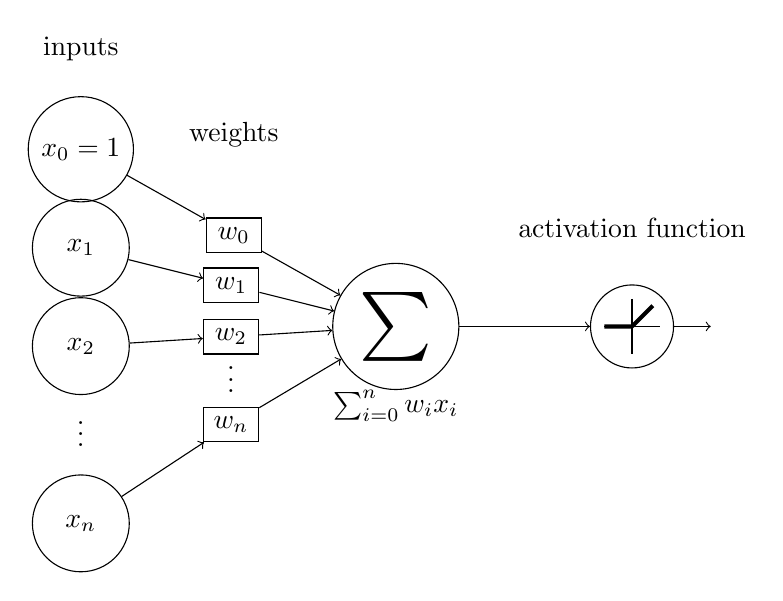
\begin{tikzpicture}
    % Draw input nodes
    \foreach \h [count=\hi ] in {$x_2$,$x_1$,$x_0=1$}{%
          \node[input] (f\hi) at (0,\hi*1.25cm-1.5 cm) {\h};
        }
    % Dot dot dot ... x_n
    \node[below=0.62cm] (idots) at (f1) {\vdots};
    \node[input, below=0.62cm] (last_input) at (idots) {$x_n$};
    % Draw summation node
    \node[functions] (sum) at (4,0) {\Huge$\sum$};
    \node[below=0.69cm] at (sum) {$\sum_{i=0}^n w_ix_i$};
    % Draw edges from input nodes to summation node
    \foreach \h [count=\hi ] in {$w_2$,$w_1$,$w_0$}{%
          \path (f\hi) -- node[weights] (w\hi) {\h} (sum);
          \draw[->] (f\hi) -- (w\hi);
          \draw[->] (w\hi) -- (sum);
        }
    % Dot dot dot ... w_n
    \node[below=0.05cm] (wdots) at (w1) {\vdots};
    \node[weights, below=0.45cm] (last_weight) at (wdots) {$w_n$};
    % Add edges for last node and last weight etc
    \path[draw,->] (last_input) -- (last_weight);
    \path[draw,->] (last_weight) -- (sum);
    % Draw node for activation function
    \node[functions] (activation) at (7,0) {};
    % Place activation function in its node
    \begin{scope}[xshift=7cm]
        \addaxes
        % flexible selection of activation function
        \relu
        % \stepfunc
    \end{scope}
    % Connect sum to relu
    \draw[->] (sum) -- (activation);
    \draw[->] (activation) -- ++(1,0);
    % Labels
    \node[above=1cm]  at (f3) {inputs};
    \node[above=1cm] at (w3) {weights};
    \node[above=1cm] at (activation) {activation function};
\end{tikzpicture}

\captionof{figure}{A single Perceptron}

\end{center}

A single basic Perceptron on its own is not particularly useful as
it only models linear decision boundaries and cannot learn the xor function \cite{MinskyPapert69}.

First we stack multiple Perceptrons to construct a layer. A layer has multiple
Perceptrons which calculate their output value with their own weights and biases on the same input values, which results
in as many output values as there are Perceptrons in the layer. Now one can construct a network which chains
multiple layers after each other, which results in a multilayer Perceptron (MLP), which is also known as a fully connected
feed forward network, as each layer is fully connected to the next layer in that each perceptron in layer $i$ 
is connected to each perceptron in layer $i+1$. The information strictly flows from input layer, through
intermediate hidden layers to the output layer, without any loops.
Mathematically a feed forward neural network, with $L$ layers and $0 < l \leq L$ can be described by

$$\mathbf{y}^{(l)} = \phi^{(l)}(\mathbf{W}^{(l)}\mathbf{y}^{(l-1)}+\mathbf{b}^{(l)})$$

where $\mathbf{W}^{(l)}$ represents the weight matrix of layer $l$, $\mathbf{b}^{(l)}$ the bias vector of layer $l$,
$\mathbf{y}^{(l-1)}$ the output vector of the previous layer or in case of $l=1$ the input vector
and $\phi^{(l)}$ is the activation function applied element-wise. \\

% TODO: is the above l=1 right?

Now the choice of the activation function is very important, when using a multilayer Perceptron as when a linear activation function like the 
identity function is used for every Percetpron the entire network can be described in a single layer. Therefore
a non-linear activation function should be used to make the network capable of learning non-linear
decision boundaries. When choosing an activation function there are some important
properties which should be respected while making such a choice. The activation function should be fully differentiable, which makes
computing the gradient easier, but is not required in all cases as workarounds can be made e.g. ReLU. It should also be computationally
cheap as its being run many times during a forward pass. \\

% TODO: some example / commonly used funcs

With loss functions the performance of a neural network on a given input can be computed by comparing the desired output with the 
predicted output of the model. Using loss functions we can quantify the error in the prediction of the neural network, which 
is a metric we can optimize for. There are again many options for choosing a loss function but it heavily depends on the nature of the
problem you're trying to solve by using a model: either classification or regression. A common loss function to use when trying to optimize 
regression tasks is the Mean Squared Error (MSE):

$$\mathcal{L}(\mathbf{y},\mathbf{\hat{y}}) = \frac{1}{n}\sum^n_{i=1}{(y_i-\hat{y}_i)^2}$$

where $\mathbf{y}$ is the prediction of the model and $\mathbf{\hat{y}}$ the ground truth. When solving classification tasks the Cross Entropy Loss function is often used:


$$\mathcal{L}(\mathbf{y},\mathbf{\hat{y}}) = -\sum^n_{i=1}{y_i\log(\hat{y}_i)}$$

With loss functions we have a metric to optimize against, which can be used in an optimization algorithm called 
gradient decent. It will minimize the loss function by iteratively computing the error gradient and updating
the weights in the opposite direction of the gradient of the loss function. This is the update rule according
to gradient decent:

$$ \theta \leftarrow \theta - \eta \nabla_{\theta}\mathcal{L}(\theta)$$

Here, $\theta$ represents the parameters, $\eta$ the learning rate that determines the size of the step we take in 
the opposite direction of the gradient and $\nabla_{\theta}\mathcal{L}(\theta)$ denotes the gradient 
of the loss function with respect to parameters $\theta$. To compute the entire gradient, all the errors for the 
entire dataset would need to be averaged for the most accurate estimation of the gradient. Therefore variants 
like stochastic gradient decent exist, that first randomizes the order of dataset, second organizes it into batches of
the same size. Now we only average the gradient for all samples inside the batch and make an update to the model parameters \cite{Bottou10}.


To actually calculating the gradient the backpropagation algorithm is used. First we take out input data and do the
forward pass to compute the predictions. We can then calculate the loss by comparing the prediction to the desired result.
Now the idea behind backpropagation is to calculate the influence of the change weights and biases to the change in loss \cite{Rumelhart86}.
Mathematically this is represented by:


$$
\frac{\partial \mathcal{L}}{\partial \mathbf{W}^{(l)}} = \frac{\partial \mathcal{L}}{\partial \mathbf{y}^{(l)}} \frac{\partial \mathbf{y}^{(l)}}{\partial \mathbf{W}^{(l)}}
$$


where $\mathcal{L}$ denotes the loss, $\mathbf{W}^{(l)}$ represents the weight matrix at layer $l$ and $\mathbf{y}^{(l)}$ stands for the output matrix
for layer $l$. Now this can be calculated at the output layer $L$ to get the error signal for the layer $L-1$. 
Then the same computation can be applied to the layer $L-1$ to propagate the error back.

\subsection{Recurrent Neural Networks}

Classic feed forward neural networks are only able to handle fix sized data, because the size of the input layer
is fixed. Sequences of variable length, like timeseries, audio or language data require a different
architecture to still being able to compute the gradients properly. This can be achieved by recurrent
neural networks (RNNs). Recurrent neural networks accomplish that by carrying a hidden state across timesteps.

\begin{center}
  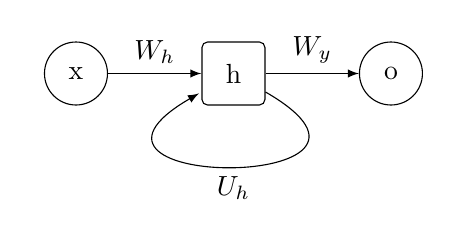
\begin{tikzpicture}[>=latex,
    % styles for clarity
    input/.style   ={draw, circle, minimum size=8mm},
    hidden/.style  ={draw, rectangle, rounded corners=2pt, minimum size=8mm},
    output/.style  ={draw, circle, minimum size=8mm},
    node distance = 2cm
  ]
    \node[input](x) at (0,0){x};
    \node[hidden](h) at (2,0) {h};
    \node[output](o) at (4, 0) {o};

    \draw[->] (x) -- node[above]{$W_h$} (h);
    \draw[->] (h) -- node[above]{$W_y$} (o);
    \path
      (h) edge[->,
            out=-30,
            in=-150,
            looseness=7,
            loop]
            node[below]{$U_h$}
      (h);
  \end{tikzpicture}
\end{center}

The RNN Cell is very similar to the Perceptron. It still has weights, biases and an activation function. Additionally 
it has a recurrent connection to itself: the output of a rnn cell at timestep $t$ is feed back to itself at timestep
$t+1$ multiplied by its own weight. That output value is called the hidden state $h_t$ of an rnn cell.
A Elman RNN is described by the forward state update and output projection \cite{Elman90}:

$$
h_t = \phi\!\bigl(W_h x_t + U_h h_{t-1} + b_h\bigr), \quad
y_t = \psi\!\bigl(W_y h_t + b_y\bigr).
$$
which can be understood as a neural network with fully connected input and output layers together with a hidden rnn layer.
The forward state update projection $h_t$ is similar to the perceptron where $b_h$ represents the bias, $W_h$ the weights,
with the addition of the term $U_hh_{t-1}$. $h_{t-1}$ is the hidden state of the last iteration and $U_h$ is the weight
matrix for the hidden state. Typically that output is then feed though a fully connected output layer map the
potentially high dimensional hidden state into the output space.\\


To calculate the gradient in a network with recurrent connections you need to unroll the network in time. The network
is unrolled over a sequence of length $T$, by creating $T$ copies of the same cell. All copies share the same weights.
The recurrent connections are now longer connected to themselves but their copy in the next copy. Unrolling converts 
the cyclic graph of a RNN into an acyclic graph, which is required for applying the standard backpropagation algorithm.
Figure~\ref{fig:rnn_unroll} depicts the unrolled network for $T=3$.

\begin{center}
  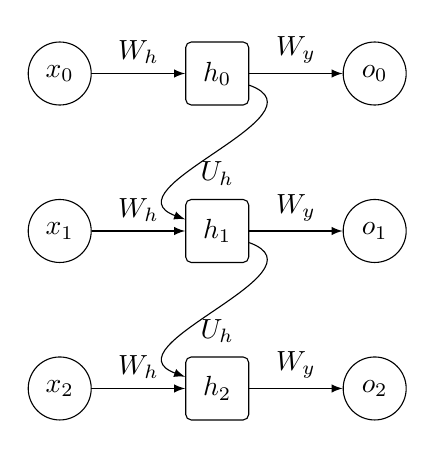
\begin{tikzpicture}[>=latex,
      % styles for clarity
      input/.style   ={draw, circle, minimum size=8mm},
      hidden/.style  ={draw, rectangle, rounded corners=2pt, minimum size=8mm},
      output/.style  ={draw, circle, minimum size=8mm},
      node distance = 2cm
    ]
    \foreach \t [count=\i from 1] in {0,1,2}{
      % place nodes at (0,-2*\i), (2,-2*\i), (4,-2*\i)
      \node[input]  (x\i) at (0,-2*\i) {$x_{\t}$};
      \node[hidden] (h\i) at (2,-2*\i) {$h_{\t}$};
      \node[output] (o\i) at (4,-2*\i) {$o_{\t}$};

      % input → hidden and hidden → output
      \draw[->] (x\i) -- node[above] {$W_h$} (h\i);
      \draw[->] (h\i) -- node[above] {$W_y$} (o\i);

      % hidden_{t–1} → hidden_t for t>0
      \ifnum\i>1
        \pgfmathtruncatemacro{\j}{\i-1}
        \draw[->, out=-20, in=160, looseness=1.5]
          (h\j) to node[below] {$U_h$} (h\i);
      \fi
    }
  \end{tikzpicture}
  \captionof{figure}{Unrolled Elman RNN for $T=3$.}\label{fig:rnn_unroll}
\end{center}




Applying backpropagation on an unrolled graph is called backpropagation through time (BPTT). On the acyclic graph 
the standard backpropagation algorithm can be applied, but the weights for all instances of the recurrent neural network
in the unrolled graph are shared. The final update for the parameter matrices are accumulated though time steps, so there 
is a contribution from everywhere a weight is used \cite{werb1990bptt}.


\subsection{Limitations of Recurrent Neural Networks}

Classic recurrent neural networks suffer from some limitations, which motivated the development 
of other RNN Variants notably LSTM networks.

\begin{enumerate}[label=(\roman*)]
\item \textbf{Vanishing and exploding gradients.}  During BPTT the gradient with respect to earlier timesteps involves products of Jacobian
  matrices $\partial h_t/\partial h_{t-1}$.  For many activation functions this product tends to shrink or blow up exponentially with
  the number of timesteps, causing the gradient norm to \emph{vanish} or \emph{explode}.
  As a consequence the network either fails to learn long‑range dependencies or becomes numerically unstable~\cite{hochreiter1997lstm,pascanu2013rnntraining}.
  Exploding gradients can be taken care of by clipping the gradient to a maximum value \cite{pascanu2013rnntraining}.
  Vanish gradients though cannot be mitigated this easily. The vanishing gradients problem is the main motivation behind the
  development of LSTM networks.
\item \textbf{Limited memory capacity.}  The entire past of the sequence must be compressed into a single hidden vector $h_t$.
  In practice the dimensionality of $h_t$ is bounded by computational constraints, creating a tight information bottleneck.
  Empirical analyses show that standard RNNs spontaneously forget information that is not constantly reinforced.
\item \textbf{Difficulty modelling very long sequences.}  Even when exploding gradients are clipped and vanishing 
  gradients mitigated, the truncation window in BPTT means the effective context length is often limited to a few hundred
  timesteps.  Tasks such as document‑level language modelling require mechanisms that can propagate information across thousands of steps \cite{pascanu2013rnntraining}.
\item \textbf{Bias towards recent inputs.}  The recurrent update $h_t=\phi(W_h x_t + U_h h_{t-1})$ blends the new input with a 
  transformed version of the previous hidden state.  Without gating, this blend is rigid and the network cannot dynamically decide 
  to \emph{copy} or \emph{forget} information.  As a result, RNNs tend to over‑weight recent inputs and under‑weight older ones.
\end{enumerate}

\section{LSTM Architecture}
\subsection{Principle of Operation (Fynn)}
\subsubsection{Intuitive Explanation}
The main goal of the LSTM architecture is to eliminate the problem of vanishing gradients. This can be achieved by ensuring a constant error flow through the network. However, when this approach is implemented naively using only a linear activation function (e.g. \begin{math}f(x)=x,\forall x\end{math}) and a weight matrix with ones on its diagonal (\begin{math}w_{jj}=1,\forall j\end{math}), problems can arise. For the inputs, a single weight can be responsible for both storing and ignoring inputs, and for the outputs, a single weight can be responsible for both allowing and preventing the distribution of a unit's memory. During training, this can result in contradictory weight update signals, affecting the network's performance. \cite{hochreiter1997lstm}\\
The solution proposed by Hochreiter and Schmidhuber introduces so-called 'gate units' at the input and output of the constant error flow to control the storage and retrieval of memory through context. This results in a structure they refer to as a 'memory cell' (often just 'cell'), as shown in Figure \ref{fig:lstm-cell}.\cite{hochreiter1997lstm}.
\begin{figure}[h!]
    \centering
    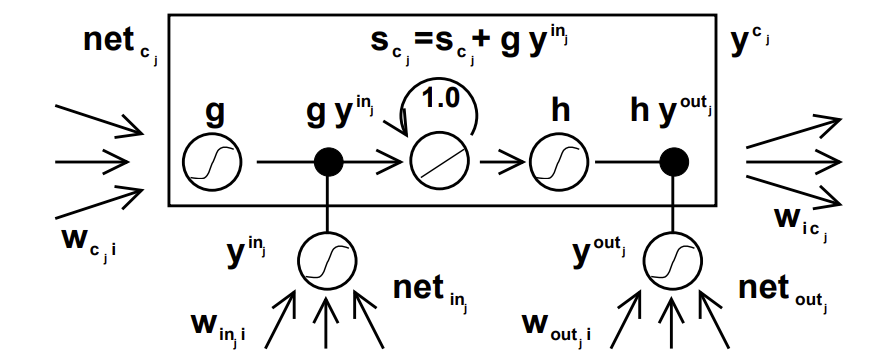
\includegraphics[width=\linewidth]{LSTM-Cell-Diagram.png}
    \caption{LSTM Cell\\ Source: \cite{hochreiter1997lstm}}
    \label{fig:lstm-cell}
\end{figure}
\\As their name suggests, gate units are used to restrict the flow of information.  The amount of gating applied to an input is determined by values computed from another input, enabling the gate to open and close depending on the context. Figure \ref{fig:lstm-cell} shows input and output gates represented by large black dots inside the cell, where input flows from left to right through the gate and control input reaches the gate from the bottom.\cite{hochreiter1997lstm}
Internally, the cell stores a state that normally starts at \begin{math}0\end{math} and to which the scaled input is added. This state is then scaled using the activation of the output gate to compute the output.
This means that an LSTM cell comprises three individual parts:\\
\textbf{Input Gate.} The input gate controls how much of the cell's input should be stored in memory, thereby determining which inputs are relevant. in the given context.\\
\textbf{Internal State.} The internal state can be viewed as the cell's memory. It is computed using the state from the previous time step to which the cell input activations, after scaling using the input gate activations are added.\\
\textbf{Output Gate.} The output gate scales the cell state before output, thereby controlling the retrieval of information from the cell.\cite{hochreiter1997lstm} \\
To improve understanding of how information flows through an LSTM cell, let us follow the flow of information through the cell at a single time step:
First, the net input for the cell and the gates is computed by multiplying the weights by the inputs (for example, the current activations of the input units and the previous output activations of the cell) and summing them. Next, the activation functions are evaluated on the gate net input activations to compute the gate activations. Then the cell net input is scaled using a function and then scaled again using the input activations. This result is then added to the internal state to update it. Finally,  the internal state is scaled using another function and then each component is scaled using the output gate activations to obtain the cell output activations.\cite{hochreiter1997lstm}
\subsubsection{Mathematical Formalization}
To formalize this approach, the activations at time t are defined as the output of the respective activation function of the net input at that time:\\
\textbf{Input gate activations:}
\begin{equation}
\label{eqn:poo-act-in}
y^{in}(t)=f_{in}\left(net_{in}(t)\right).
\end{equation}
\textbf{Output gate activations:}
\begin{equation}
\label{eqn:poo-act-out}
y^{out}(t)=f_{out}\left(net_{out}(t)\right)
\end{equation}
\textbf{Cell output activations:}
\begin{equation}
\label{eqn:poo-act-c}
y^{c}(t)=y^{out}(t)h\left(s_c(t)\right)
\end{equation}
where \begin{math}s_c\end{math} is the "internal state" of the cell, given by:
\begin{equation}
\label{eqn:poo-state0}
s_c(0)=0
\end{equation}
\begin{equation}
\label{eqn:poo-state}
s_c(t)=s_c(t-1)+y^{in}(t)g\left(net_c(t)\right)
\end{equation}
and the net inputs \begin{math}net_{in}(t), net_{out}(t)\end{math} and \begin{math}net_c(t)\end{math} are the sum of the result of multiplying the weight matrix with the activations from the previous time step for all different inputs:\\
\textbf{Input gate net input:}
\begin{equation}
\label{eqn:poo-net-in}
net_{in}(t)=\sum_{u}{w_{in\ u}}y^u(t-1).
\end{equation}
\textbf{Output gate net input:}
\begin{equation}
   \label{eqn:poo-net-out}
   net_{out}(t)=\sum_{u}{w_{out\ u}}y^u(t-1).
\end{equation}
\textbf{Cell net input:}
\begin{equation}
   \label{eqn:poo-net-c}
   net_{c}(t)=\sum_{u}{w_{c\ u}}y^u(t-1).
\end{equation}
The values of the summation index \begin{math}u\end{math} represent the different inputs and depend on the chosen network architecture. These values can represent input units, memory cells, gate units, or hidden units from this or other cells.
The function \begin{math}g\end{math} is used to scale the cell net input before gating, and the function \begin{math}h\end{math} is used to scale the memory cell output before gating.
Note that multiplying two vectors together does not give the dot product, but rather the Hadamard product, which multiplies vectors component-wise.\cite{gokmen2018hadamard} This allows each component of the vector to be gated individually.
An index \begin{math}j\end{math} can be added to identify individual cells. This has been omitted here to make the notation easier to read.\cite{hochreiter1997lstm}

\subsection{Example Implementation (Fynn)}
\subsubsection{Network Architecture}
Before implementing a simple LSTM network, the network architecture must first be defined.
For simplicity, the activations for the cell, input gate and output gate will be the output activations, as well as the activations of the input units:   \begin{math}u\in\{c, x, b \}\end{math}, where \begin{math}y^c(t)\end{math} are the output activations at time \begin{math}t\end{math}, \begin{math}y^x(t-1)=x(t)\end{math} are the activations of the input units at time \begin{math}t\end{math} and \begin{math}y^b(t-1)=b\end{math} are the bias units.\cite{hochreiter1997lstm}\\ 
As the biases are constant, we can define \begin{math}b_u=w_{u\ b}b\end{math} and use those individual biases as weights to reduce the total number of weights.
This means that the sums describing the inputs for the input gate, output gate, and cell  (see equations \ref{eqn:poo-net-in}, \ref{eqn:poo-net-out}, and \ref{eqn:imp-net-c})  can be written as follows:
\begin{equation}
\label{eqn:imp-net-in}
net_{in}(t)=w_{in\ c}y^c(t-1)+w_{in\ x}x(t)+b_{in},
\end{equation}
\begin{equation}
\label{eqn:imp-net-out}
net_{out}(t)=w_{out\ c}y^c(t-1)+w_{out\ x}x(t)+b_{out}
\end{equation}
\begin{equation}
\label{eqn:imp-net-c}
net_c(t)=w_{c\ c}y^c(t-1)+w_{c\ x}x(t)+b_c.
\end{equation}
\subsubsection{Implementing the Network}
The PyTorch library is used for the implementation of the network. To keep things simple, the input and output will always be vectors of the same length given by the parameter \lstinline{size}.\\
Firstly, a class that extends \lstinline{torch.nn.Module} s defined, along with its attributes: the input/output size of the cell; the weight matrices \begin{math}w_{in\ c},w_{in\ x},w_{out\ c},w_{out\ x},w_{c\ c},w_{c\ x}\end{math}; and the biases \begin{math}b_{in},b_c,b_{out}\end{math}:\cite{keras-lstm,pytorch-lstm}
\begin{lstlisting}
class LSTMCell(torch.nn.Module):
    
    size : int # Input Size (1D)
    
    w_i_c : torch.Tensor # Input gate weights
    w_i_x : torch.Tensor # Input gate weights
    w_c_c : torch.Tensor # Cell input weights
    w_c_x : torch.Tensor # Cell input weights
    w_o_c : torch.Tensor # Output gate weights
    w_o_x : torch.Tensor # Output gate weights
    
    b_i : torch.Tensor # Input gate biases
    b_c : torch.Tensor # Cell input biases
    b_o : torch.Tensor # Output gate biases
\end{lstlisting}
When a new object of the class is created, the weights should be randomized, as shown in (a), and the biases should be initialized to zero, as shown in (b). All of these should also be marked as trainable parameters, which can be achieved by using \lstinline{torch.nn.Parameter}:\cite{keras-lstm,pytorch-lstm}
\begin{lstlisting}
def __init__(self, size : int):
    super(LSTMCell, self).__init__()
    self.size = size
    
    # Initialize weights (a)
    self.w_i_c = torch.nn.Parameter(torch.randn(size, size) * 0.01)
    self.w_i_x = torch.nn.Parameter(torch.randn(size, size) * 0.01)
    self.w_c_c = torch.nn.Parameter(torch.randn(size, size) * 0.01)
    self.w_c_x = torch.nn.Parameter(torch.randn(size, size) * 0.01)
    self.w_o_c = torch.nn.Parameter(torch.randn(size, size) * 0.01)
    self.w_o_x = torch.nn.Parameter(torch.randn(size, size) * 0.01)
    
    # Initialize weights biases (b)
    self.b_i = torch.nn.Parameter(torch.zeros(size))
    self.b_c = torch.nn.Parameter(torch.zeros(size))
    self.b_o = torch.nn.Parameter(torch.zeros(size))   
\end{lstlisting}
Next, the activation functions are defined based on those used in the Hochreiter and Schmidhuber experiments. The functions\begin{math}f, g\end{math} and \begin{math} h \end{math} are given as follows: \cite{hochreiter1997lstm}
\begin{equation}
    \label{eqn:imp-f}
    f(x)=\frac{1}{1+\exp(-x)},
\end{equation}
\begin{equation}
\label{eqn:imp-g}
    g(x)=\frac{4}{1+\exp(-x)}-2
\end{equation}
\begin{equation}
    \label{eqn:imp-h}
    h(x)=\frac{2}{1+\exp(-x)}-1.
\end{equation}
For function \begin{math}f\end{math} (see \ref{eqn:imp-f}, \lstinline{torch.sigmoid} is used, as it is a standard sigmoid function. The functions \begin{math}g\end{math} and \begin{math}h\end{math} (see \ref{eqn:imp-g}, \ref{eqn:imp-h}) are just scaled and shifted sigmoid functions, they can be implemented by multiplying the result of the sigmoid function with a scalar, and subtracting a tensor of the same shape as the input, set to either \begin{math}1\end{math}'s (see (c)) or \begin{math}2\end{math}'s (see (d)) entirely:\cite{hochreiter1997lstm, pytorch-lstm}
\begin{lstlisting}
@staticmethod
def _f(x: torch.Tensor) -> torch.Tensor:
    return torch.sigmoid(x)
@staticmethod
def _g(x: torch.Tensor) -> torch.Tensor:
    return torch.sigmoid(x) * 4 - torch.ones_like(x) * 2 # (c)
@staticmethod
def _h(x: torch.Tensor) -> torch.Tensor:
    return torch.sigmoid(x) * 2 - torch.ones_like(x) # (d)
\end{lstlisting}
These can then be used to implement a function that forwards an input through the cell. This function takes the current input, as well as the cell's previous output and state, and returns the cell's output and current state. To compute the outputs, the input \lstinline{x_t} must first be converted to a vector if it is a scalar (see (e)), so that the matrix multiplication operator can be used in the case \lstinline{size == 1}:\cite{keras-lstm, pytorch-lstm}
\begin{lstlisting}
def forward(self, x_t : torch.Tensor, y_tm1 : torch.Tensor, c_tm1 : torch.Tensor) -> tuple[torch.Tensor, torch.Tensor]:
    if x_t.dim() == 0:  # x_t is scalar (e)
        x_t = x_t.unsqueeze(0)
\end{lstlisting}
Using equations \ref{eqn:imp-net-in} and \ref{eqn:imp-net-out}, the net input for the input, as well as the input and output gates, can be calculated, as shown at (f) and (h). This can then be passed through the function f (see equation \ref{eqn:imp-f}) to obtain the respective gate activations, as shown at (g) and (i) (see equation  \ref{eqn:poo-act-in} and \ref{eqn:poo-act-out}):\cite{hochreiter1997lstm, keras-lstm, pytorch-lstm}
\begin{lstlisting}
# Input gate activations
net_i = self.w_i_c @ y_tm1 + self.w_i_x @ x_t + self.b_i # (f)
y_i   = self._f(net_i)                                   # (g)
        
# Output gate activations
net_o = self.w_o_c @ y_tm1 + self.w_o_x @ x_t + self.b_o # (h)
y_o   = self._f(net_o)                                   # (i)
\end{lstlisting}
Using those, the cell net input is computed using equation \ref{eqn:imp-net-c} as is implemented at (j). 
The cell state is computed using equation \ref{eqn:poo-state} as is done at (k) and the cells output using equation \ref{eqn:poo-act-c} as is done at (l). Finally the output and cell state are returned, for the next time step:\cite{hochreiter1997lstm,keras-lstm, pytorch-lstm}:
\begin{lstlisting}
# Compute cell input
net_c = self.w_c_c @ y_tm1 + self.w_c_x @ x_t.squeeze() + self.b_c # (j)
c_t = c_tm1 + y_i * self._g(net_c) # Update cell state               (k)
y_t = y_o * self._h(c_t)           # Compute output                  (l)
        
return y_t, c_t
\end{lstlisting}
\subsubsection{Testing the implementation}
To test whether the implementation works, two LSTM cells are created: one with a size of 1 and one with a size of 20. An input matching the size of each cell is then passed through them:\cite{pytorch-lstm}
\begin{lstlisting}
lstm1 = LSTMCell(1)
lstm1(torch.zeros(1), torch.zeros(1), torch.zeros(1)) # x_t, y_tm1, c_tm1
lstm20 = LSTMCell(20)
lstm20(torch.zeros(1), torch.zeros(1), torch.zeros(1))
\end{lstlisting}
This code executes without throwing any errors, implying that all the tensors are the intended size and that there are no other critical errors in the implementation.\\
Next, the performance is tested on a sequence of values sampled from the function \begin{math}\sin(2\pi t)\end{math}. 
First, the function for generating the sequence is defined with parameters for noise and sample lag. This outputs a list containing two elements: the sampled value and the time difference to the previous value. This time difference is constant if no sampling lag is applied:
\begin{lstlisting}
def genSequence(length : int, dt : float = 0.05, noise = 0, samplingLag = 0) -> list[list[float]]:
    t = 0
    result = []
    for i in range(length):
        tm1 = t
        t = t + dt + samplingLag * random.uniform(-1, 1) * dt
        x = math.sin(2 * math.pi * t) + noise * random.uniform(-1, 1)
        result.append([x, t - tm1])
    return result
\end{lstlisting}
The model is defined, as an LSTM cell with a size of 2. The loss function chosen is Mean Absolute Error, as it is typically used for regression tasks like this and so the loss of errors \begin{math}<1\end{math} is not squished and ADAM is chosen as the optimizer, as it works well for LSTMs:\cite{chang2018adamlstm,willmott2005losses,terven2025losses}
\begin{lstlisting}
model = LSTMCell(2)
loss_fn = torch.nn.L1Loss()  # L1Loss for regression tasks 
optimizer = torch.optim.Adam(model.parameters(), lr=0.0015)
\end{lstlisting}
Finally, the train function can be implemented:
\begin{lstlisting}
def train(epochs : int, batches : int, batch_size : int):
    data = genSequence(batch_size * batches, samplingLag=0.0, noise=0.0)
    for epoch in range(epochs):
        total_loss = 0.0
        for n in range(batches):
            # Zero gradient and batch_loss (m)
            optimizer.zero_grad() 
            batch_loss = 0.0
            
            # Get batch data # (n)
            batch = torch.tensor(data[n * batch_size : (n + 1) * batch_size])    
            # Initialize internal state and input (o)
            c_t = torch.zeros(model.size)
            y_t = torch.zeros(model.size)
            
            # Compute output and loss for each time step and add up all the losses (p)
            for t in range(batch_size - 1):
                input = batch[t]
                target = batch[t + 1]
                y_t, c_t = model(input, y_t, c_t)
                loss = loss_fn(y_t[0], target[0])
                batch_loss += loss      
            # Calculate the average the batch loss and backpropogate it (q)
            batch_loss /= (batch_size - 1)  # Average loss for the batch
            total_loss += batch_loss.item()
            batch_loss.backward()
            
            # Gradient clipping, to avoid expoloding gradients
            # and adjust parameters (r)
            torch.nn.utils.clip_grad_norm_(model.parameters(), 1.0)
            optimizer.step() 
        avg_loss = total_loss / batches
        print(f"Epoch {epoch + 1}/{epochs}, Average Loss: {avg_loss:.4f}")
        loss_graph.gca().plot(epoch, avg_loss, 'ro')
\end{lstlisting}
\begin{figure}[h!]
    \centering
    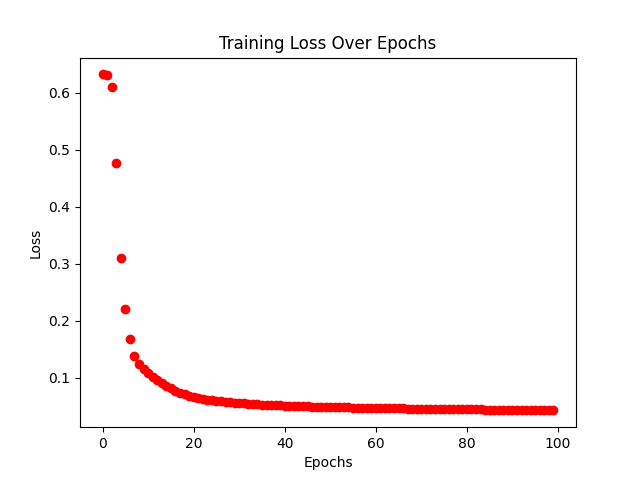
\includegraphics[width=0.75\linewidth]{train_loss_graph.png}
    \caption{Training loss}
    \label{fig:train-loss-graph}
\end{figure}
The function first generates a sequence and then trains the network on all batches for the specified number of epochs. For each batch the first step is to zero the gradient and batch loss as done at (m). Next the batch is retrieved from the sequence and converted to a tensor as done at (n). Then the internal state is set to zero, as required by Equation \ref{eqn:poo-state0} and the cell's current output is set to zero as well as done at (o). Next, the output and loss at each time step are computed and summed up for each time step, as is done at (p). This is archived, by passing each input in the batch into the network and updating the cell state and the cell output so they can be used as inputs at the next time step. Afterwards the average of the batch is calculated by dividing by the batch size, and this average gets back-propagated through the network, as is done at (q). Finally at (r), the gradients are clipped to avoid exploding gradients, and the models parameters are adjusted. An average of the current batch loss is also computed, which is printed for monitoring training and added to a plot for visual analysis.\cite{werb1990bptt, pytorch-rnn, gradient-clipping, pascanu2013rnntraining, hochreiter1997lstm}  
\\Training the network for 100 epochs, with 100 batches of size 125 each, results in the graph Figure \ref{fig:train-loss-graph}, which shows a typical curve for training a neural network, with a steep drop-off at the start, which then settles to a value.\cite{training-graphs}
The decrease in the loss function indicates successful training. Due to the L1Loss, the Average Loss is \begin{math}\ell_a=\overline \ell_b\end{math} where the average batch loss \begin{math}\ell_b=\overline{\left|d(t)-y^c(t)\right|}\end{math}, meaning it is the average of the average batch loss over all batches, where the average batch loss is the average of the absolute value of the difference between expected output and the networks output. Because the loss is directly proportional to the difference between target and output, small and large errors are weighted equally in training.\\
Now the network is tested by predicting a sequence with different lengths. For this a sequence is first generated, the  cell state and cell output initialized with zero, and then the network is called and the loss computed similarly as to how it was done when training the network:
\begin{lstlisting}
seq, y_t, c_t = genSequence(25), torch.zeros(model.size), torch.zeros(model.size)
for t in range(0, 24):
    x_t = torch.tensor(seq[t])
    y_t, c_t = model(x_t, y_t, c_t)
    test_graph.gca().plot(t, loss_fn(y_t[0], torch.tensor(seq[t+1][0])).item(), 'bo')
\end{lstlisting}

\begin{figure}[h!]
    \centering
    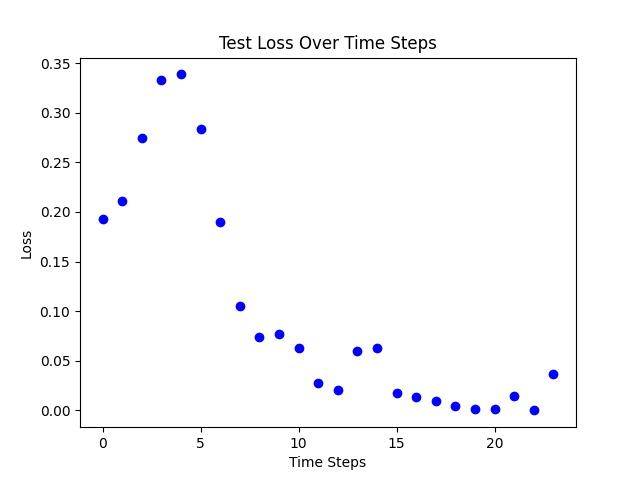
\includegraphics[width=0.75\linewidth]{test_loss_graph.png}
    \caption{Test sequence loss}
    \label{fig:test-loss-graph}
\end{figure}
The loss at each timestep is added to the plot shown in Figure \ref{fig:test-loss-graph}. The plot clearly shows that the network struggles to predict the next value for short input sequences, but its performance improves as the sequence gets longer, which is typical for LSTMs. \cite{bolboaca2023lstmperformance} Overall, the predicted values never deviate by more than \begin{math}0.35\end{math} from the targets.\\
Next, the performance is tested with noise and sampling lag added by simply adjusting the \lstinline{noise} and \lstinline{samplingLag} parameters in the train function and test sequence.
\begin{figure}[h!]
    \centering
    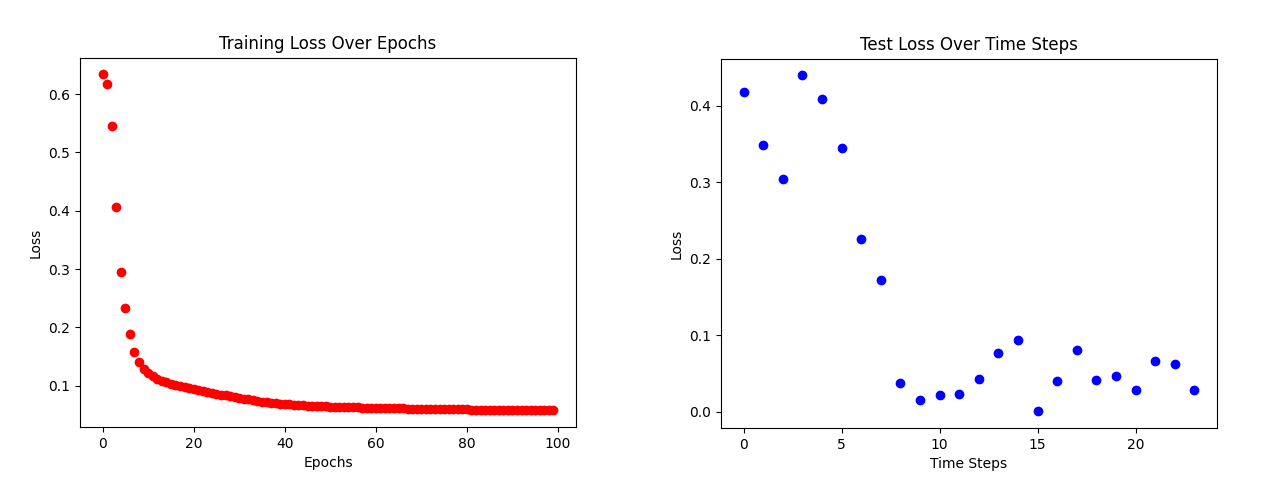
\includegraphics[width=\linewidth]{loss_with_noise.png}
    \caption{Losses with 10\% sampling lag and 5\% noise added to data}
    \label{fig:loss-noise}
\end{figure}
\\The resulting graphs, shown in Figure \ref{fig:loss-noise}, demonstrate that the model's performance is only slightly worse than on data with no noise. The loss during training settles at a slightly higher value and the loss during testing is about \begin{math}0.1\end{math} higher for short sequences and  \begin{math}0.05\end{math} higher for longer sequences.\\
\textbf{Possible Improvements:} As the input is a repeating sequence of values, the implementation could be improved by introducing a forget gate. This would allow the network to predict the next values without needing to consider the entire previous sequence.\cite{gers1999forgetgate}\\
Another way to get a better performance would be to use a Gated recurrent unit (GRU) instead of an LSTM, as GRUs often perform better with short sequences.\cite{cahuantzi2023lstmvsgru}
\section{Limitations and Alternatives}

\subsection{Limitations (Fynn)}
Although LSTMs solve some of the problems associated with classical RNNs, they also have some disadvantages, including:
\begin{itemize}
    \item \textbf{Computational Intensity:} Computational intensity: As an LSTM cell requires additional weights for the gates, the number of weights can increase by up to a factor of \begin{math} 9 \end{math}. However, this is usually not a significant issue, as LSTM networks typically have a similar number of weights to other RNNs.\cite{hochreiter1997lstm}\\ However, in applications that require low power, such as mobile devices, this could cause problems. \cite{rizakisFPGAlstm}
    \item \textbf{Exploding Gradients:} Although the LSTM architecture mitigates the issue of vanishing gradients, it does not eliminate that of exploding gradients.\cite{pascanu2013rnntraining} This can be achieved using alternative techniques, such as gradient clipping.\cite{gradient-clipping, pascanu2013rnntraining}
    \item \textbf{Limited GPU utilization and memory bottlenecks:} LSTM networks do not utilize the GPU fully and tend to train less efficiently on modern GPUs. Furthermore, they are often limited by the available GPU memory.\cite{zheng2018scalability, zheng2020scalability}  
    \item \textbf{Worse performance on less complex sequences:} Although LSTMs perform better than some other architectures, such as GRUs, on sequences with high complexity, they struggle more on simpler sequences.\cite{cahuantzi2023lstmvsgru} 
    \item \textbf{Worse performance on short sequences:} As discussed in Section 4.2.3, LSTMs tend to perform poorly with short sequences, often achieving significantly higher loss. \cite{bolboaca2023lstmperformance} 
\end{itemize}

\subsection{Variants}

\subsubsection{LSTM with Forget Gate (Fynn)}
\begin{figure}[h]
    \centering
    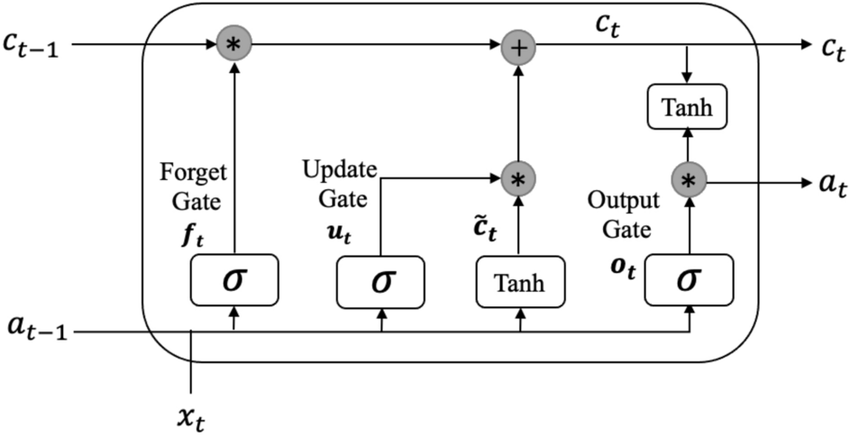
\includegraphics[width=0.75\linewidth]{Structure-of-LSTM-cell-which-introduces-three-special-gates-Input-Gate-i-Forget-Gate.png}
    \caption{LSTM Cell with forget gate\\ Source: \cite{nguyen2022lstmforgetgraphic}}
    \label{fig:lstm-forget}
\end{figure}
One of the first variation of Hochreiter and Schmidhuber's architecture, was the introduction of a forget gate. The reason for its introduction is that there is no way for the internal state of the cell to be reset in the original architecture. To fix this a forget gate can be introduced, which restricts how much of the previous state is kept in the next time step.\cite{gers1999forgetgate}\\
Figure \ref{fig:lstm-forget} shows an LSTM cell, with the added forget gate on the left of the cell. Note that the input gate is labeled as "Update Gate" in this graphic.\\
The forget gate is implemented like the other with\cite{gers1999forgetgate}
\begin{equation}
    net_\varphi(t)=\sum_uw_{\varphi\ u}y^u(t-1)
    \label{eqn:forget-net-in}
\end{equation}
and
\begin{equation}
    y^\varphi(t)=f_\varphi\left(net_\varphi(t)\right).
    \label{eqn:forget-actiavtions}
\end{equation} 
Equation \ref{eqn:forget-net-in} describes the net inputs for the forget gate, and equation \ref{eqn:forget-actiavtions} describes the activation for the forget gate. Using those a new equation for the cell state can be defined as\cite{gers1999forgetgate}
\begin{equation}
    s_c(t)=y^\varphi(t)s_c(t-1)+y^{in}(t)g\left(net_c(t)\right).    
\end{equation}
  This addition is very common, and many LSTM implementations in commonly used machine learning frameworks include a forget gate.\cite{keras-lstm, pytorch-lstm}
 \subsubsection{Coupled Input-Forget Gate}

\subsubsection{Simplified LSTM}

\subsubsection{LSTM with Attention}

\subsubsection{Bidirectional LSTM}

\subsubsection{Deep LSTM}

\subsubsection{Zoneout LSTM}

Examines notable variants discussing their respective enhancements and capabilities.
(Approximately 1-1.5 pages, written by Leon/Fynn)
% TODO:

\subsection{LSTM vs GRU}

\subsection{LSTM vs Transformers (Leon)}

\section{Applications}

\subsection{Natural Language Processing (Leon)}

We have already established that LSTM networks are great at working with sequence data. One example where LSTM networks
have been successfully used is speech recognition. The LSTM network learns temporal patterns in audio and captures long 
term relationships. They have achieved state of the art results in a paper by Google in 2014 \cite{sak2014longshorttermmemorybased}.
Researchers at google showed that a deep LSTM network outperformed traditional deep neural networks for this problem.
It was even better then a feed forward neural network with 10x more parameters \cite[1]{sak2014longshorttermmemorybased}.
They used an LSTM variant called Long Short-Term Memory Projected (LSTMP) architecture \cite[2]{sak2014longshorttermmemorybased} which 
outperformed the traditional LSTM architecture. The LSTMP architecture differs from the traditional LSTM one by not having a LSTM layer
which output is directly connected to its input but they first do a linear projection with a fully connected layer and its output will represent the 
hidden state of the cell.

\subsection{Time Series Forecasting (Fynn)}
While LSTMs can be used to forecast time series, they often are inferior to other methods.\cite{gers2001timeseries} But for certain applications, like speech or music, they are a better choice, as they perform better on more complex sequences.\cite{gers2001timeseries, cahuantzi2023lstmvsgru}\\
In a 2022 article by Torres, they use an deep LSTM network, to predict electricity demands and achieve errors of just \begin{math}1.5\%\end{math}.\cite{torres2022elctricityforecasting}\\
Kılıç et al. (2024) uses the LSTM architecture to predict electricity prices, and achieve better results compared to other architectures.\cite{nielsen2024electricitypriceforcasting}

\subsection{Music and Audio (Fynn)}
As mentioned in the introduction, music has structures and patterns, where the next note or chord depends on the previous ones. LSTMs can learn those patterns and predict what comes next, which allows them to generate music.\cite{eck2002musicgeneration}\\
In their 2002 paper Eck and Schmidhuber use an LSTM network to generate chord progressions, as well as melodies and chord progressions. Their network successfully managed to pick up on patterns in a style of music and reproduce those patterns to compose new music in the same style.\cite{eck2002musicgeneration}  
\subsection{Medical (Leon)}

\section{Conclusion (Fynn)}
The LSTM architecture introduced gate units and memory cells, effectively eliminating the vanishing gradient problem that had prevented RNNs from reaching their full potential.\cite{hochreiter1997lstm} 
This enabled LSTMs to be used for tasks such as time series forecasting, music generation, and natural language processing.\cite{eck2002musicgeneration,nielsen2024electricitypriceforcasting,gers2001timeseries,torres2022elctricityforecasting,sak2014longshorttermmemorybased}\\
Although LSTMs have been replaced by architectures such as transformers in many applications, they are still useful because they perform better with small datasets. This is why further research into improving the performance of this architecture is likely.\cite{alselwi2024lstmfuture} Furthermore, they will likely form the basis of new architectures. For example, LSTM-Transformer hybrid architectures already exist today. \cite{zhao2025lstmtransformerhybrid} 
\bibliographystyle{alpha}
\bibliography{abbrev,seminar_report}
\end{document}
